\begin{figure*}[t]
  \centering
  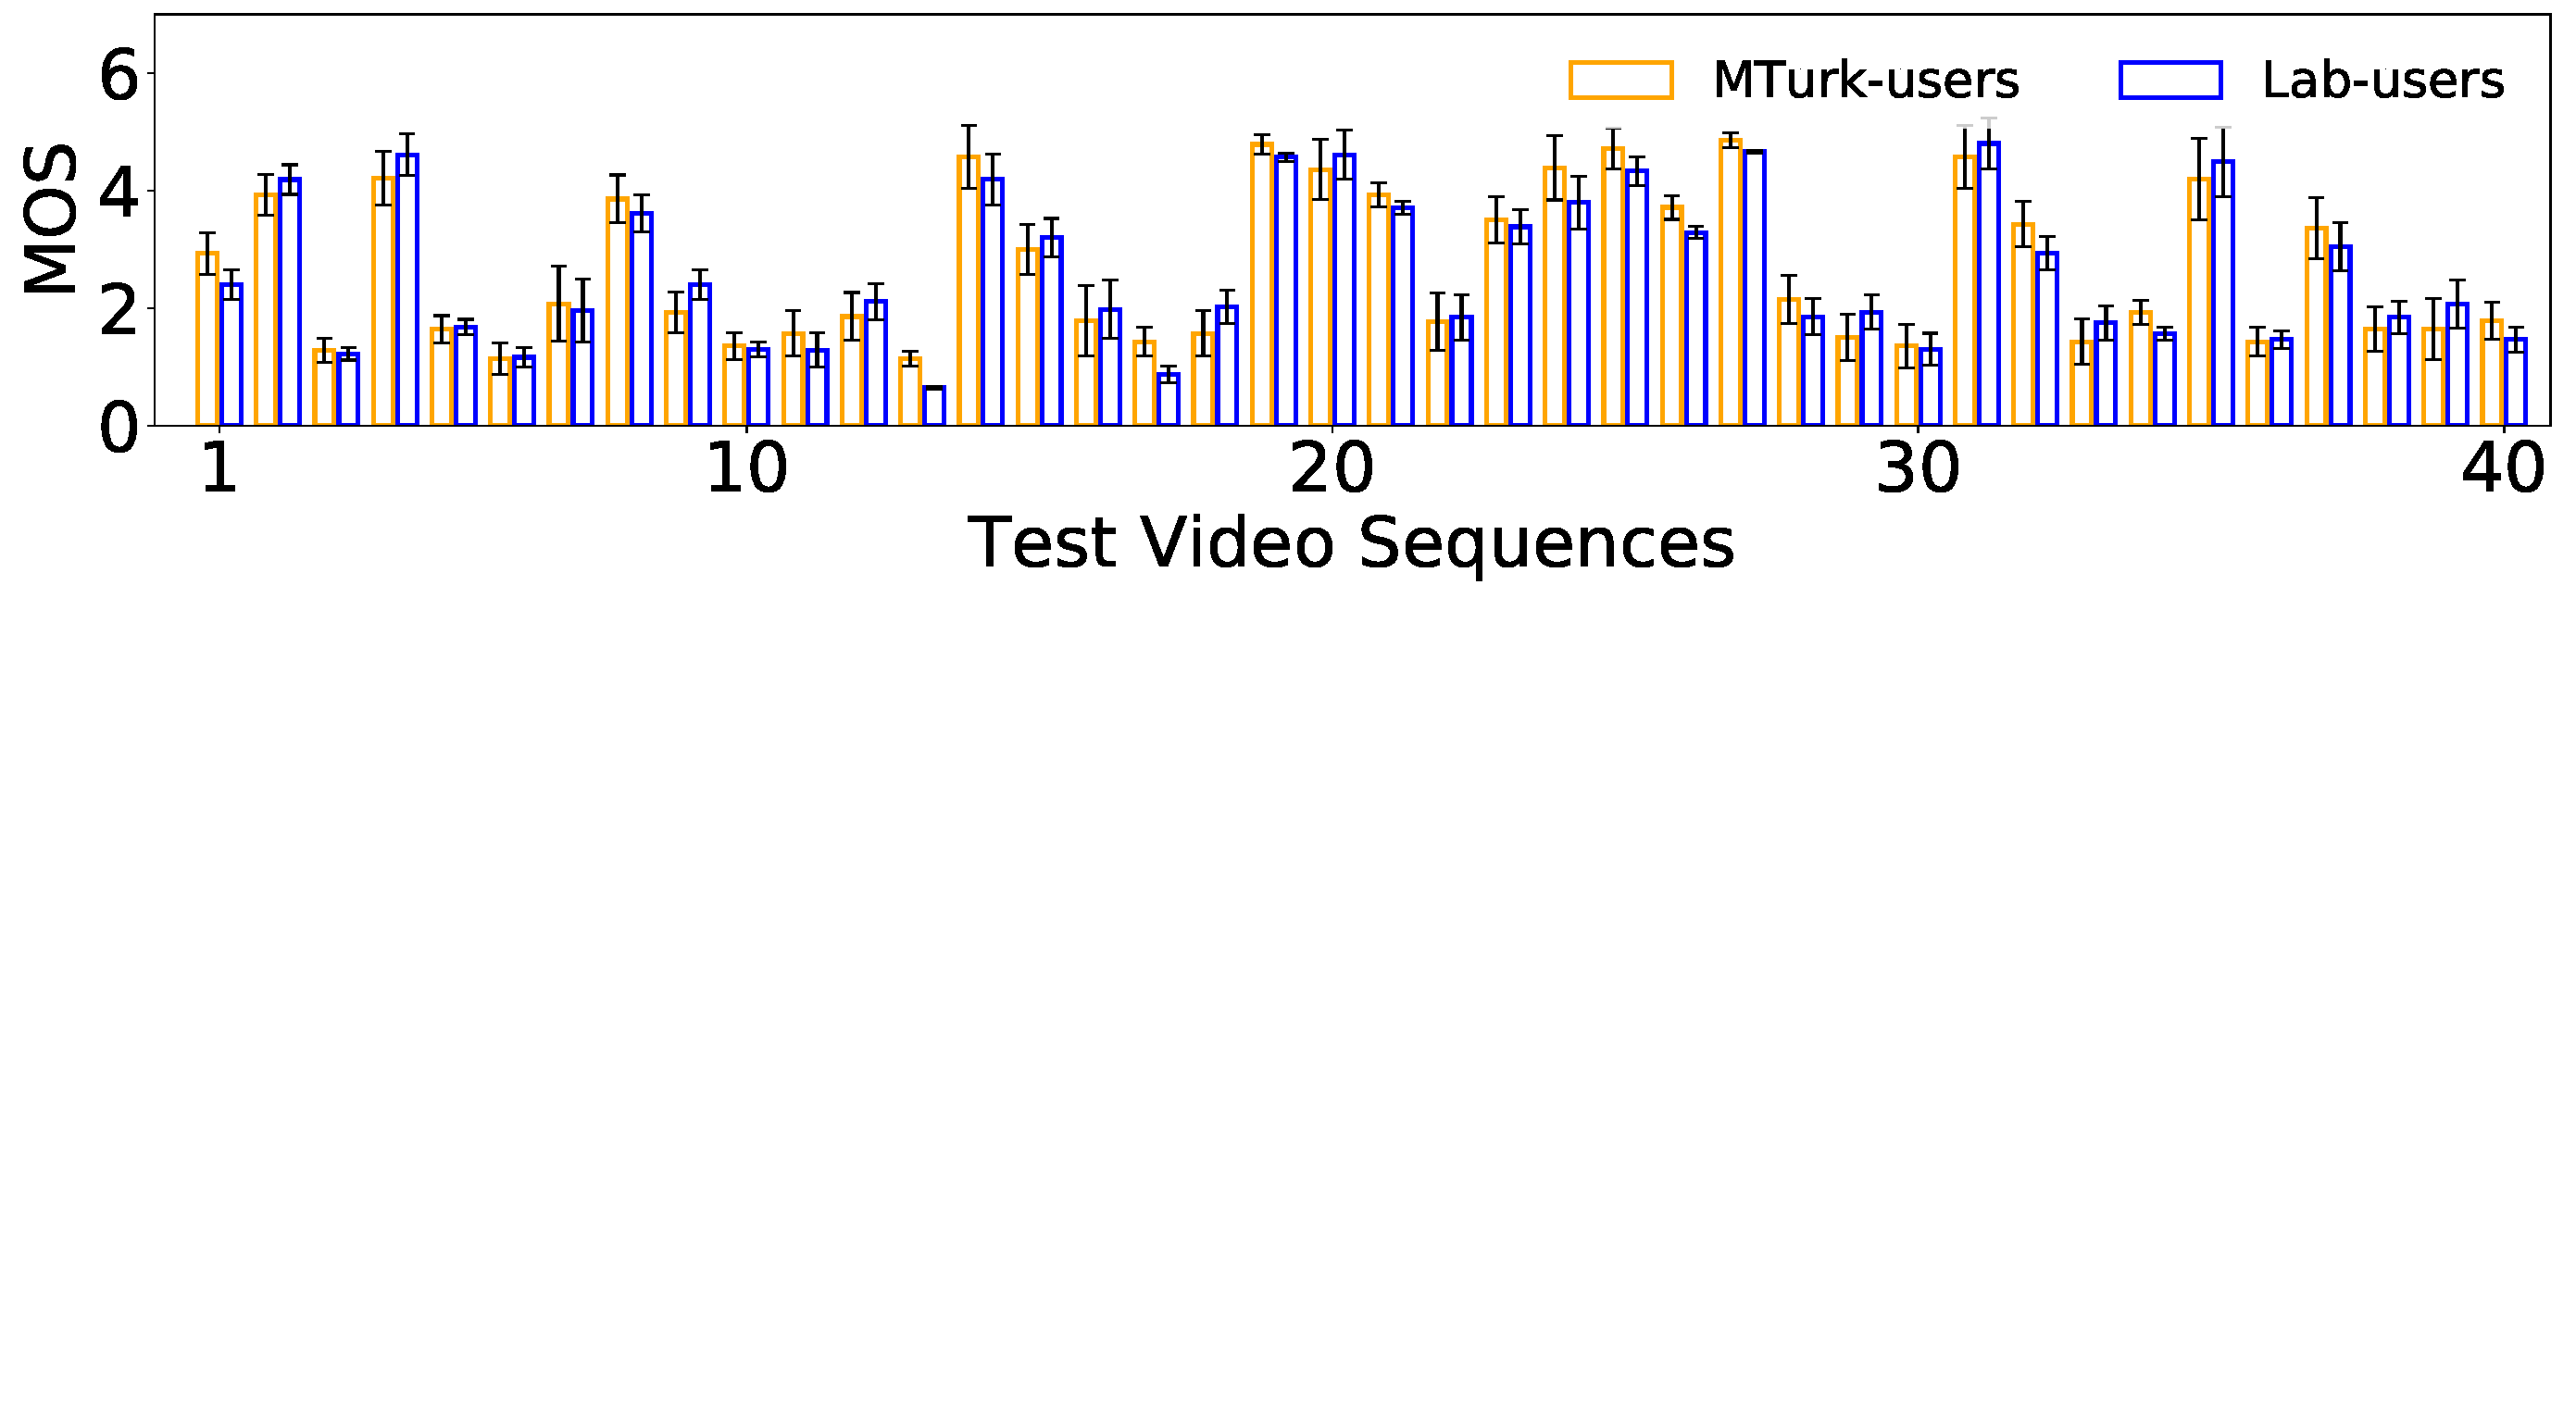
\includegraphics[width=0.8\textwidth]{sections/network-work/mos}
  \vspace{-2in}
  \caption{MOS and standard deviation of QoE scores from 30 lab and 30 online users. Although the scores vary across the users both in lab and online, the distribution of MOS is similar in two cases.}
  \vspace{-0.15in}
  \label{fig:mos}
\end{figure*}

\section{From Video Artefacts to Q\lowercase{o}E} \label{label:results}
We validate our QoE metrics presented in Section~\ref{label:design} with subjective measurements. We seek to ensure that our metrics accurately capture  video telephony QoE artefacts. Video artefacts vary across applications and network conditions. Additionally, they can appear together (e.g., when we have both blurriness and stutter) or independently. Intermingled video artefacts result in diverse QoE levels (from bad to excellent), standardized as MOS by ITU-T~\cite{series2012methodology}\footnote{MOS takes values from 1 to 5, with 5 being excellent.}. We carry out a user study and obtain a MOS for each video.

\subsection{Data Preparation}
As described in Section \ref{label:design}, the dataset is prepared from recorded video calls. We use 20 videos described in Section \ref{MOTIVATION}, for video calls on Skype, FaceTime and Hangouts. For each video and application, we repeat  experiments on  multiple devices. The video calls are recorded under different network conditions to produce good, average and bad quality videos. We record video calls for Skype, Hangouts on Samsung Galaxy (SG) S6 edge, Google Pixel Tab, SG S2 Tab and for FaceTime on iPad Pro (model A1674) and iPhone 8 Plus. We post-process these videos into 30 seconds  video clips and evaluate QoE for each clip. We host a web server with these video clips and ask the users to rate their experience after watching each sample. 

\subsection{User-Study Setup}
We conduct the user-study in two phases: 1) in two labs, 2) online using a crowd sourced platform. The lab user study is conducted at a university campus and an enterprise lab. The online user study is conducted on Amazon Mechanical Turk platform \cite{turk-amazon}. Online users are from the United States and are in age range 20--40. We collect results from 60 lab users and more than 150 online users\footnote{Our conducted user-studies are approved by the Institutional Review Board (IRB) of our institution. Evidence to be provided upon paper acceptance.}. We faced several challenges  while deploying a user-study in the wild, such as ensuring that 1) users watch the whole video clip without fast forwarding and then rate their experience, 2) users can rate the video if and only if they watch the video, 3) users watch on screens of similar size  to avoid huge QoE variance i.e., small screen users do not perceive poor quality compared to large screen users. We address these challenges by carefully designing the user-study website and avoiding noisy samples. First, we disable the video controls in the web page so that users cannot advance the video. Second, we introduce random attention pop-up buttons while watching the video and ask users to click on the attention button to confirm that they are watching the video. A user cannot move to next video until the current video is rated. Finally, we restrict users from taking the study on mobile devices, to avoid variance due to small screens. The user-study web page can be run on Chrome, Firefox and Safari. Once the user completes rating all the videos, results are pushed to our server. Then, users are granted a server-generated code  for processing payments in MTurk. Amazon MTurk restricts users from taking again the same study, thus our users are unique.

\subsection{Lab  vs.~MTurk Users}
We compare the MOS across lab and online users for the same set of 40 video clips and we find similar distributions across 80 clips. Fig. \ref{fig:mos} shows the MOS bar plots of user ratings. The lower the rating is, the lower the QoE is. For each video sequence, we plot the average MOS across users with error bars for standard deviation. We observe that lab and online users exhibit similar distributions of MOS. The standard deviation of MOS between lab and online users is smaller than 1 MOS for 96\% of videos. 
%In both studies, we observe lot of variance for first few videos because the users were not shown original videos. The users learn the score for each video after watching few videos and rate them correctly from then on. So we remove these intial set of videos which have high standard deviation from our data analysis. 
%Further, we also observe certain content such as videos with large portion of uniform background, have difficulty in identifying good or average case video.  %%%CHRISTINA: this sentence needs rewriting "videos have difficult in identifying?"
We find that 4\% of these video clips have more than 1 MOS standard deviation and we remove them from our analysis as outliers. Such videos have a  large portion of uniform background, hence their content challenges classification between average and good MOS.
